\section{Tests für Ladegeschwindigkeiten}
\label{sec:test_fur_ladegeschwindigkeiten}
% 3-4 Unterschiedliche Testingtools für die Ladegeschwindigkeit aufführen

% auf die unterschiedlichen Arten von Tests 


\subsection{GT Metrix}
\label{sec:gt_metrix}
GT Metrix (GTMetrix | Website Performance Testing and Monitoring, o. D.) ist ein automatisiertes Tool, das speziell für die Analyse der Ladegeschwindigkeit und der allgemeinen Performance von Websites entwickelt wurde. GT Metrix bietet eine detaillierte Analyse, die es ermöglicht, Schwachstellen zu identifizieren und gezielte Verbesserungen vorzunehmen.

Das Tool ist in einer kostenlosen und einer kostenpflichtigen Version verfügbar, wobei bereits die kostenlose Version zahlreiche Funktionen bietet. Ein besonders wichtiger Bestandteil der Analyse sind die so genannten "Core Web Vitals", die im Suchalgorithmus von Google eine entscheidende Rolle spielen. Diese Metriken, die die Ladezeit, die Interaktivität und die visuelle Stabilität einer Seite bewerten, sind entscheidend für die Platzierung einer Website in den Suchergebnissen von Google. GT Metrix erstellt nach jedem Test einen umfassenden Bericht, der sowohl die Performance der Website als auch ihre strukturellen Merkmale aufzeigt. Der Performance Score ist ein Maß für die Performance der Website aus Sicht des Nutzers, der Structure Score ein Maß dafür, wie gut die Website für eine optimale Performance strukturiert ist.

Zusätzlich bietet GT Metrix eine visuelle Darstellung der Ladegeschwindigkeit in Form der "Speed Visualisation". Dabei wird der Ladevorgang der Seite in Intervallen dargestellt und wichtige Leistungsindikatoren während des Ladevorgangs hervorgehoben. So kann der Nutzer den Ladevorgang besser nachvollziehen und erkennen, welche Bereiche der Seite besonders viel Zeit in Anspruch nehmen. Darüber hinaus listet das Tool im Abschnitt "Top Issues" strukturelle Probleme auf, die zu den größten Leistungsverlusten führen, so dass die größten Schwachstellen der Website leicht identifiziert werden können. Die "Page Details" sind eine Aufschlüsselung der Anfragen, die während des Seitenaufrufs gestellt wurden, einschließlich der Anzahl und Größe dieser Anfragen. Diese detaillierte Übersicht gibt Aufschluss darüber, welche Elemente der Website den Seitenaufbau verlangsamen können.

Basierend auf der durchgeführten Analyse liefert das Tool auch konkrete Optimierungsvorschläge. Diese Vorschläge sind in einem eigenen GT Metrix-Bereich zusammengefasst und helfen dem Nutzer, gezielt an den identifizierten Schwachstellen zu arbeiten. Die verschiedenen Reiter für Performance, Struktur und weitere Bereiche ermöglichen eine detaillierte Betrachtung der Testergebnisse. Besonders praktisch ist die Möglichkeit, die Website-Performance aus verschiedenen geografischen Regionen zu testen. Sieben globale Standorte ermöglichen es dem Nutzer zu sehen, wie schnell seine Seite in verschiedenen Teilen der Welt geladen wird.

Ein weiteres nützliches Feature der kostenlosen Version ist die Möglichkeit, automatisierte Tests zu planen, die täglich, wöchentlich oder monatlich ausgeführt werden. Damit lassen sich langfristige Trends wie die Entwicklung der Web Vitals, des GT Metrix Grades, der Performance- und Struktur-Scores, der Seiten- und Dateigrößen sowie der Anzahl der Requests verfolgen. Auf diese Weise ist der Website-Betreiber in der Lage, die Performance seiner Website über einen längeren Zeitraum zu beobachten und frühzeitig auf Veränderungen zu reagieren.

Ein weiterer wichtiger Bestandteil der Analyse ist das Wasserfalldiagramm, das den Ladeprozess der Seite detailliert darstellt und lange oder fehlerhafte Requests hervorhebt. Diese visuelle Darstellung hilft, Engpässe im Ladeprozess zu identifizieren und gezielt Verbesserungen vorzunehmen. Darüber hinaus bietet GT Metrix die Möglichkeit, Tests mit und ohne Adblocker durchzuführen, um zu sehen, wie Werbung die Ladezeiten beeinflusst. Eine Verbindungsdrosselungsfunktion ermöglicht es, die Performance der Website bei unterschiedlichen Internetgeschwindigkeiten zu simulieren. Weitere Funktionen der kostenlosen Version sind Benachrichtigungen, wenn die Performance unter ein bestimmtes Niveau fällt, und die Möglichkeit, den Ladevorgang der Website aus Sicht des Nutzers per Video Playback zu sehen.

Die kostenpflichtige Version von GT Metrix erweitert den Funktionsumfang der kostenlosen Version erheblich und bietet zahlreiche zusätzliche Tools, die insbesondere für fortgeschrittene Nutzer und Unternehmen nützlich sind. Eine der wichtigsten Erweiterungen ist das Mobile Testing, mit dem die Performance einer Website auf über 40 verschiedenen Mobilgeräten getestet werden kann, darunter beliebte Modelle wie iPhone, Samsung Galaxy und Google Pixels. Dies ist wichtig, da immer mehr Nutzerinnen und Nutzer von mobilen Geräten aus auf Websites zugreifen und eine optimale Performance auf diesen Geräten unerlässlich ist.

Darüber hinaus bietet die kostenpflichtige Version 15 zusätzliche globale Standorte, die es ermöglichen, die Ladegeschwindigkeit und Performance der Website in noch mehr geografischen Regionen zu testen. Dies erweitert die Reichweite im Vergleich zu den sieben Standorten der kostenlosen Version erheblich und ist besonders für international ausgerichtete Websites hilfreich, die ihre Nutzer in verschiedenen Teilen der Welt erreichen möchten.

Ein weiteres leistungsstarkes Feature ist die stündliche Überwachung der Website-Performance. Damit lassen sich detaillierte Informationen darüber gewinnen, zu welchen Tageszeiten die größten Leistungseinbußen auftreten. Dies ermöglicht eine genauere Diagnose von Problemen und gibt Einblick in das Nutzerverhalten zu unterschiedlichen Zeiten.

Darüber hinaus bietet die kostenpflichtige Version eine unbegrenzte Anzahl von Tags, die zur Kategorisierung und Sortierung von Fehlern und Berichten verwendet werden können. Diese Funktion ist besonders nützlich, um wiederkehrende Probleme zu verwalten und zu organisieren oder um einen systematischen Überblick über Bereiche mit Verbesserungspotenzial zu erhalten. Weitere erweiterte Analyseoptionen umfassen die Anpassung der Bildschirmauflösung und der Internetgeschwindigkeit, um noch genauere Tests durchzuführen und die Ladezeiten unter verschiedenen Bedingungen zu simulieren.

Ein zusätzlicher Vorteil der Premium-Version ist die längere Speicherung der Berichte, die einen tieferen Einblick in die vergangene Leistung der Website bietet und langfristige Trends besser sichtbar macht. Für Entwickler, die in einer Entwicklungs- oder Staging-Umgebung arbeiten, bietet die kostenpflichtige Version auch die Möglichkeit, einen eigenen DNS zu verwenden. Damit können Hostnamen und IP-Adressen für spezifische Testzwecke angepasst werden.

Ein weiterer Vorzug der kostenpflichtigen Version ist der priorisierte Zugriff auf die Warteschlange der Benutzeranfragen, was eine schnellere Bearbeitung der Tests und eine schnellere Bereitstellung der Ergebnisse ermöglicht. Die Möglichkeit des weltweiten Monitorings und der Download kompletter PDF-Berichte bieten eine umfassende Dokumentation der Testergebnisse, die leicht weitergegeben und archiviert werden kann.

Ein weiteres zentrales Feature der Premium-Version ist die API-Funktionalität. Diese ermöglicht es Entwicklern und Unternehmen, GT Metrix direkt in ihre eigenen Systeme zu integrieren und automatisierte Tests sowie detaillierte Analysen durchzuführen. Mit der API können Performancetests ohne manuelle Eingriffe durchgeführt werden, was insbesondere bei größeren Projekten oder für ein regelmäßiges Monitoring von Vorteil ist. Mit Hilfe der API kann der gesamte Prozess automatisiert und an die individuellen Anforderungen angepasst werden. Dies spart Zeit und Ressourcen und stellt sicher, dass die Performance der Website kontinuierlich überwacht und optimiert wird. 



\subsection{Tool 2}
\label{sec:}


\subsection{Google PageSpeed Insights}
\label{sec: pagespeed_insights}

Google PageSpeed Insights basiert auf zwei verschiedenen Arten von Daten, den Felddaten und den Labordaten, die jeweils unterschiedliche Aspekte der Website-Leistung aufzeigen und zusammen ein vollständiges Bild des Nutzererlebnisses und der Ladegeschwindigkeit ergeben.

Die Felddaten in Google PageSpeed Insights stammen aus dem Chrome User Experience Report (CrUX) und sind sehr nützlich, da sie auf echten Nutzerdaten basieren, die weltweit in Chrome-Browsern erfasst wurden. Diese Daten spiegeln die tatsächliche Nutzererfahrung wieder, da sie aus realen Interaktionen von Nutzern stammen, die die Website besucht haben. Dies bedeutet, dass die Daten im Gegensatz zu simulierten Labortests ein authentisches Bild davon vermitteln, wie sich eine Website in verschiedenen Netzwerken, auf verschiedenen Geräten und unter verschiedenen Bedingungen verhält. Die Datenerhebung erfolgt in regelmäßigen Abständen, konkret alle 28 Tage, so dass die Ergebnisse kontinuierlich aktualisiert werden.

Voraussetzung für die Datenerhebung mit CrUX ist allerdings, dass die analysierte Website öffentlich zugänglich ist und über eine ausreichend große Nutzerbasis verfügt. Nur so kann eine repräsentative Stichprobe erreicht werden. Eine genaue Mindestzahl an Besuchern wird von Google nicht genannt, es wird jedoch sichergestellt, dass genügend Daten für eine valide Analyse zur Verfügung stehen. Ein weiterer wichtiger Aspekt der Felddaten ist, dass sie zwischen mobilen Geräten und Computern unterscheiden, um die Performance in beiden Nutzungsszenarien genau abbilden zu können.

\begin{figure}
    \centering
    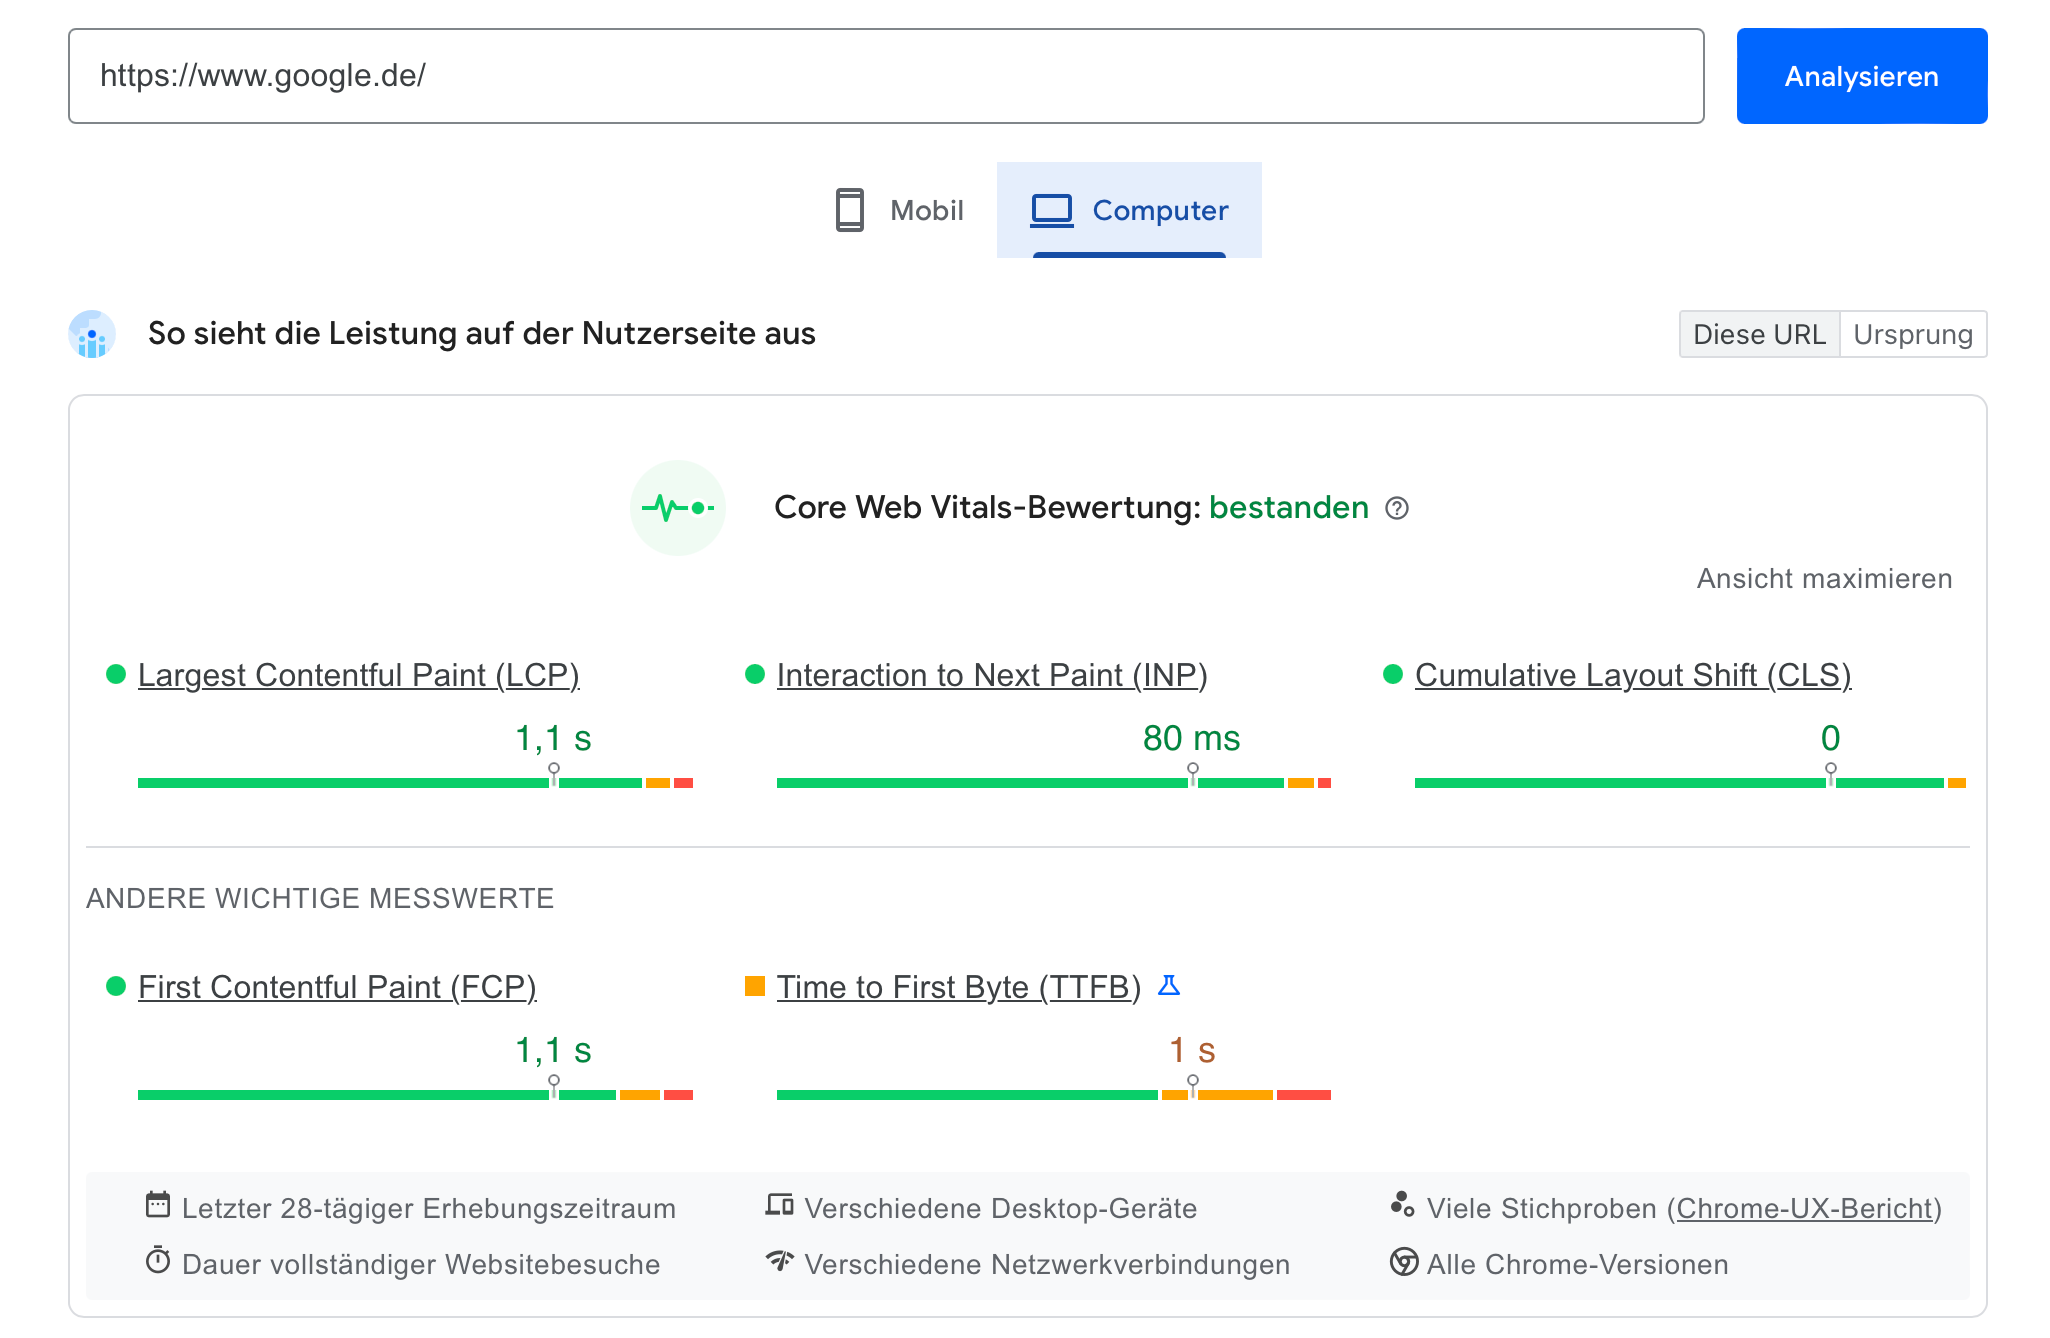
\includegraphics[width=1 \textwidth]{psi_user}
    \caption{PageSpeed Insights Übersicht der CrUX-Daten am Beispiel von https://www.google.de/}
    \label{fig:crux_data}
\end{figure}

Für die Analyse der Website-Performance werden mehrere Leistungskennzahlen gemessen, die wichtige Informationen über die Ladegeschwindigkeit und das Nutzererlebnis liefern. Eine der zentralen Metriken ist "Largest Contentful Paint" (LCP), welche den Zeitpunkt misst, zu dem der größte sichtbare Inhalt einer Seite geladen wird. Dies ist besonders relevant, da die Nutzer erwarten, dass sie schnell zum Hauptinhalt einer Seite gelangen. Ein weiterer wichtiger Indikator ist Interaction to Next Paint (INP), welcher die Reaktionsfähigkeit der Seite auf Nutzerinteraktionen während der Nutzung misst. Diese Metrik gibt Aufschluss darüber, wie gut die Seite auf Benutzereingaben reagiert, was ein wichtiger Faktor für die Benutzererfahrung ist.

Cumulative Layout Shift (CLS) ist eine Metrik, die Layoutverschiebungen während des Seitenladens misst. Unerwartete Bewegungen von Inhalten, wie das Verschieben von Text oder Bildern, können das Nutzererlebnis negativ beeinflussen, daher ist der CLS-Wert wichtig, um die visuelle Stabilität der Seite zu beurteilen. Zusätzlich wird der First Contentful Paint (FCP) gemessen, der den Zeitpunkt angibt, zu dem der Nutzer den Inhalt der Seite zum ersten Mal sieht. Ein schneller FCP sorgt für einen positiven ersten Eindruck, da der Nutzer sofort eine visuelle Rückmeldung erhält, dass die Seite geladen wird. Die Time to First Byte (TTFB) gibt schließlich an, wie lange es dauert, bis der Browser die ersten Daten vom Server erhält. Eine niedrige TTFB ist ein Zeichen für einen schnellen Server und eine effiziente Backend-Infrastruktur.

Die Lab-Daten in Google PageSpeed Insights stammen aus Lighthouse, einem Open-Source-Tool von Google, das Webseiten unter kontrollierten Bedingungen analysiert. Im Gegensatz zu den Field-Daten, die reale Nutzerdaten wiederspiegeln, werden die Lab-Daten in einer simulierten Umgebung erhoben. Das bedeutet, dass die Performance der Seite unter bestimmten, vordefinierten Bedingungen getestet wird. Dies geschieht durch die Emulation von Geräten und Netzwerkbedingungen, um möglichst realitätsnahe Szenarien zu simulieren. So wird beispielsweise ein Moto G Power als Standardgerät für mobile Tests verwendet und die Netzwerkgeschwindigkeit künstlich gedrosselt, um zu simulieren, wie die Seite unter langsameren Verbindungen geladen wird.

Lab-Daten liefern eine Momentaufnahme der aktuellen Leistung einer Website und konzentrieren sich auf die Seite, wie sie zum Zeitpunkt der Messung existiert. Im Gegensatz zu den Felddaten wird hier nicht auf historische Nutzerdaten zurückgegriffen, sondern die jeweilige URL wird einmalig getestet. Es werden nur die explizit eingegebenen URLs analysiert, nicht aber die angrenzenden Seiten, wie es beispielsweise bei CrUX der Fall ist.

Die Ergebnisse der Lab-Daten werden in vier Kategorien eingeteilt: Performance, Accessibility, Best Practices und SEO (Search Engine Optimization). Für die Analyse der Ladegeschwindigkeit ist vor allem die Kategorie Performance relevant. In dieser Kategorie bewertet PageSpeed Insights die Performance der Seite anhand von fünf wichtigen Schlüsselmetriken, die in einen Performance-Score einfließen.

\begin{figure}
    \centering
    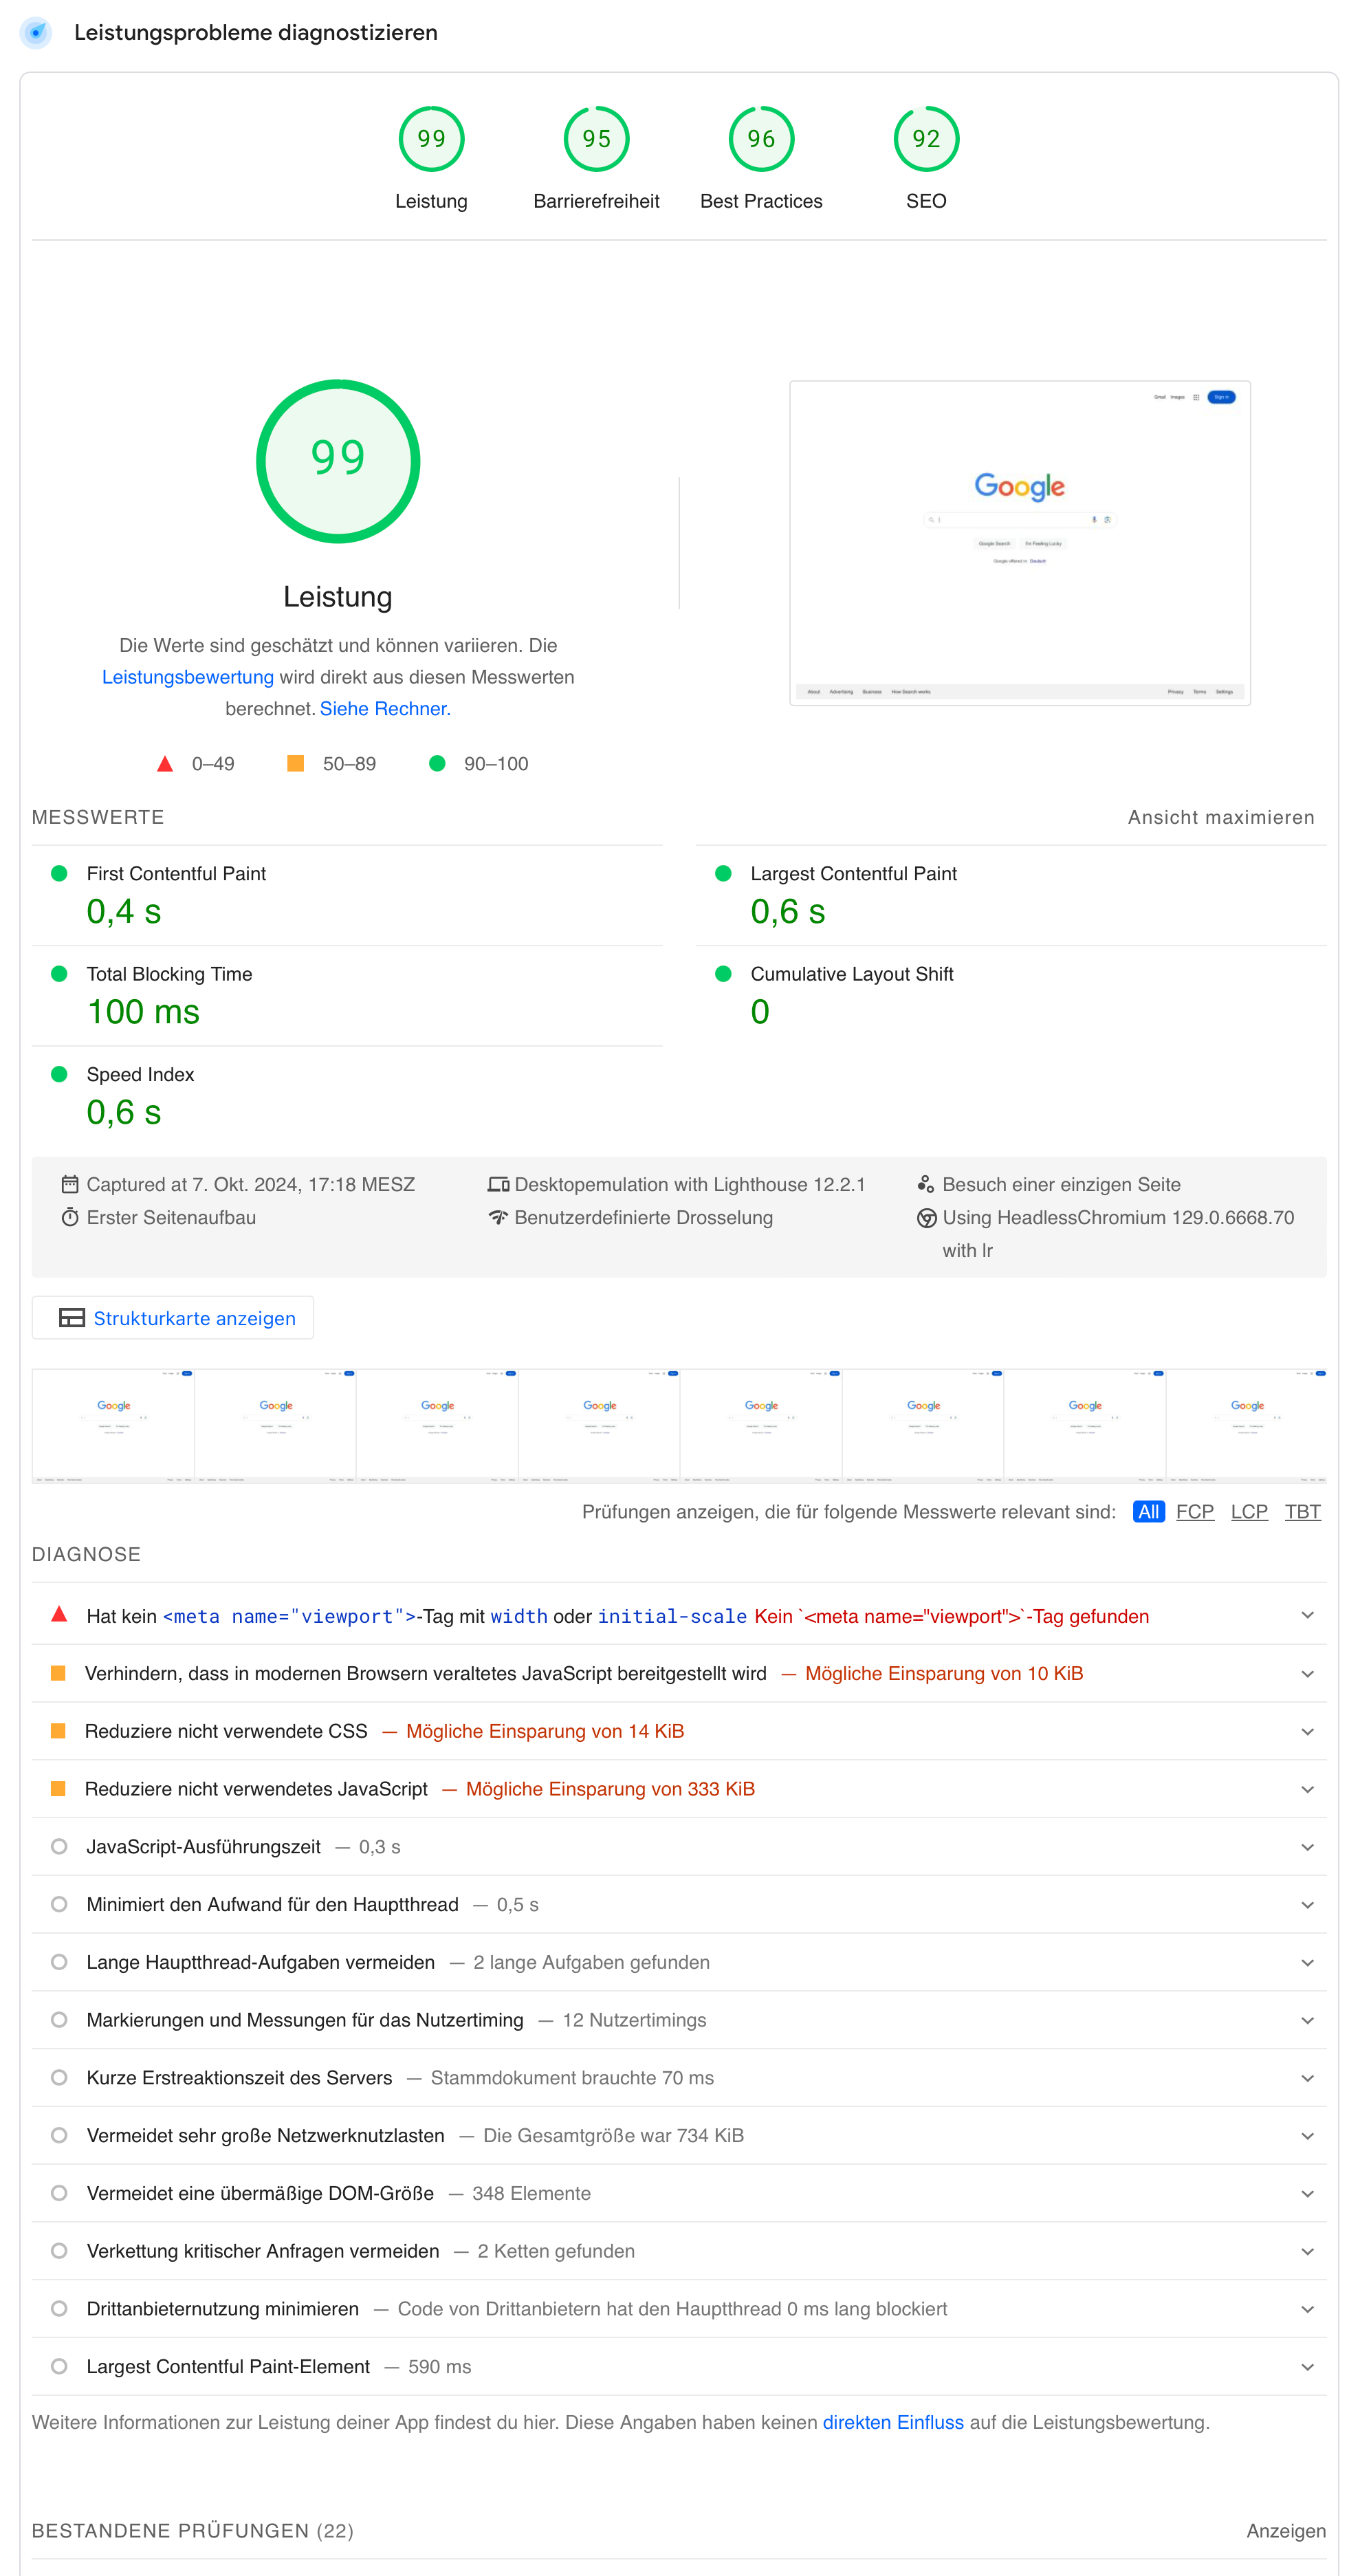
\includegraphics[height=0.9\textheight]{psi_performance}
    \caption{PageSpeed Insights Übersicht der Lab-Daten am Beispiel von https://www.google.de/}
    \label{fig:psi_performance}
\end{figure}

Zu diesen Metriken gehört wie bei CrUX  First Contentful Paint (FCP), Largest Contentful Paint (LCP) und Cumulative Layout Shift (CLS), welche nochmals zum Zeitpunkt der Anfrage ermittelt werden. 

Eine weitere wesentliche Metrik ist die Total Blocking Time (TBT). Sie misst die Summe der Zeiträume, in denen die Seite blockiert ist und nicht auf Benutzerinteraktionen reagiert. Dieser Wert ist besonders wichtig, um festzustellen, ob die Seite in der Lage ist, schnell auf Benutzereingaben zu reagieren, was einen großen Einfluss auf die allgemeine Benutzererfahrung hat. Schließlich gibt es noch den Speed Index, der angibt, wie schnell der Inhalt einer Seite insgesamt angezeigt wird.

Zusätzlich zu diesen Kernmetriken bietet Lighthouse auch detaillierte Informationen über die Seitenstruktur und visualisiert den Aufbau der Website in einer Reihe von Bildern, die zeigen, wie die Seite Schritt für Schritt geladen wird. Diese visuelle Darstellung kann helfen, Engpässe im Ladeprozess zu identifizieren. Zusätzlich gibt es den Reiter Diagnose, der mögliche Probleme auflistet und Einsparpotenziale aufzeigt. Diese Diagnosehinweise enthalten  konkrete Vorschläge zur Verbesserung der Ladegeschwindigkeit und zur Behebung von Schwachstellen.

Abgerundet wird die Analyse durch bestandene Tests, die zeigen, welche Tests die Seite ohne Probleme bestanden hat. 

Ein weiterer großer Vorteil von Google PageSpeed Insights ist die Verfügbarkeit einer kostenlosen API, über die Entwickler und Website-Betreiber automatisiert auf die Messwerte zugreifen können. Diese API ermöglicht es, regelmäßige Performance-Tests durchzuführen, ohne manuell auf die PageSpeed Insights-Website zugreifen zu müssen. Besonders nützlich ist die Möglichkeit, zusätzliche Daten wie Time to Interactive, DOM Size und Total Byte Weight abzufragen, um eine noch detailliertere Analyse der Performance durchzuführen. Mit einem API-Schlüssel können bis zu 240 Abfragen pro Minute bzw. 25.000 Abfragen pro Tag kostenlos durchgeführt werden.

PageSpeed Insights ist generell kostenlos und ohne Login für jeden zugänglich. Durch die Kombination von realen Nutzerdaten und Lab-Daten bietet Google PageSpeed Insights einen umfassenden und zuverlässigen Einblick in die Ladegeschwindigkeit und allgemeine Performance einer Website. In meiner empirischen Analyse im späteren Verlauf der Arbeit wird Google PageSpeed Insights als zentrales Tool verwendet, um die Ladegeschwindigkeit und Performance verschiedener Websites zu analysieren.

